% DEPRECATED !!!

% \subsection{Influência Social e seus Efeitos} \label{sec:socialinfluence}

% Segundo \citeonline{Simons-Morton2010}, a influência social representa o efeito que outros causam sobre os comportamentos e atitudes de indivíduos ou grupos. A influência pode originar-se tanto de pessoas muito próximas, com as quais o invidíduo em questão possui um relacionamento íntimo, quanto de pessoas mais distantes, com as quais existe um laço social direto porém o mesmo não é muito intenso \cite{Berkman2000}. Entretanto, até mesmo pessoas desconhecidas podem causar algum nível de influência; uma demonstração deste fenômeno foi relatada na pesquisa de \citeonline{Fowler2008}, que identificou que a disseminação de felicidade em uma rede estudada durante 20 anos se estende por até três graus de separação (ou seja, pode advir de amigos de amigos de amigos). Na figura \ref{fig:socialzones}, tem-se uma representação das zonas de contato social entre indivíduos.

% \begin{figure}
%     \centering
%     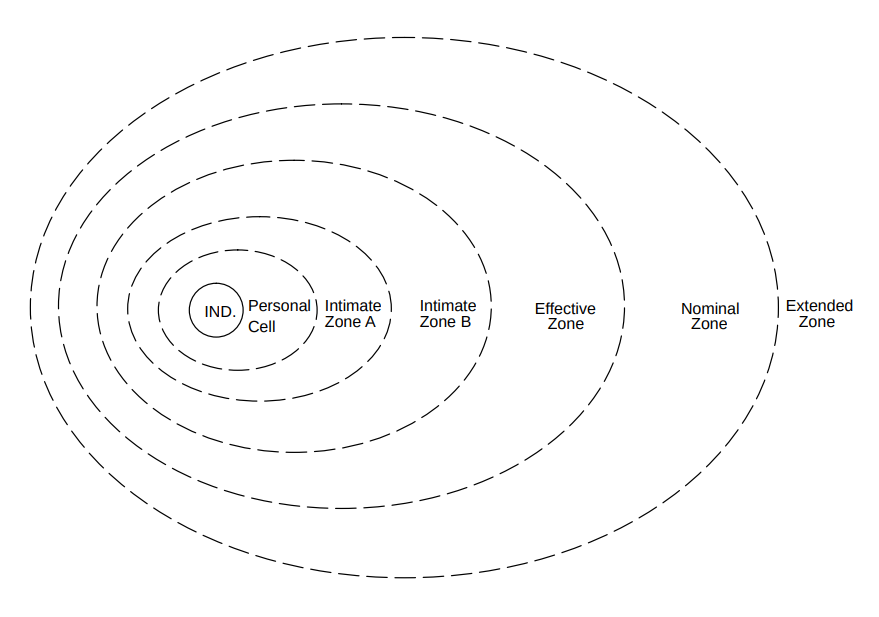
\includegraphics[width=12cm]{imagens/zones.png}
%     \caption{Zonas de contato social. Fonte: \cite{Berkman2000}}
%     \label{fig:socialzones}
% \end{figure}

% O modelo apresentado pela figura foi descrito por \citeonline{Berkman2000} com base em outros estudos sobre influência social e níveis de contato. Neste modelo, tem-se seis zonas sociais: (i) \textit{personal cell} (célula pessoal), que representa os familiares mais próximos e os mais íntimos dos amigos; (ii) \textit{intimate zone A} (zona íntima A), que representa familiares próximos e amizades íntimas ativas; (iii) \textit{intimate zone B} (zona íntima B), que consiste em familiares e amigos emocionalmente importantes mas com um cunho mais passivo; (iv) \textit{effective zone} (zona efetiva), composta por pessoas com as quais o relacionamento é mantido devido a razões de necessidade cotidiana; (v) \textit{nominal zone} (zona nominal), que contém apenas pessoas que o indivíduo conhece mas que não apresentam grande importância; e (vi) \textit{extended zone} (zona estendida), que consiste em pessoas distantes com as quais não há quase nenhum contato, porém o indivíduo em questão as conhece pelo menos de rosto.

% \citeonline{Berkman2000} argumenta que todas as zonas do modelo apresentam importância considerável, não somente os círculos mais internos. Apesar de estes serem extremamente importantes para a manutenção da saúde emocional, indivíduos que pertencem à zona efetiva, nominal ou estendida fornecem suporte instrumental -- ou seja, auxiliam na execução de alguma tarefa ou na conquista de algum objetivo. Assim, tais indivíduos podem causar mudanças de comportamento e portanto também são agentes de influência social, mesmo que de forma menos acentuada.

% Tratando das consequências da influência social, \citeonline{Steinberg2007} relatam que, assim como outros estudos conduzidos previamente evidenciaram, a adoção de hábitos perigosos e nocivos -- como abuso de substâncias, delinquência e imprudência no trânsito -- aumenta significativamente no período da adolescência, primariamente devido à maior susceptibilidade a pressão de pares, e estabiliza à medida que o indivíduo atinge a idade adulta.

% Entretanto, este padrão também se mantém para condutas neutras ou até mesmo socialmente valorizadas, como tirar notas boas ou evitar drogas. Os autores sugerem que tal comportamento pode ser causado pela noção de que os pares de um indivíduo representam um ponto de referência comportamental que deve ser seguido, caracterizando o grupo social como um ambiente que tende à homogeneidade -- em caso de visões conflitantes, o indivíduo que foge à regra pode sofrer uma série de efeitos negativos, como rejeição, ostracismo e exclusão do grupo \cite{Steinberg2007}.

% \subsection{Redes Sociais no Contexto Educacional} \label{sec:networkseducation}

% A influência social e a disseminação de comportamento também causam profundos efeitos sobre os hábitos de estudantes, especialmente devido à grande quantidade de tempo que estes passam interagindo com seus colegas de classe, sendo esta uma característica observada principalmente no período da adolescência \cite{Butler-Barnes2015}. Na literatura científica, tem-se um considerável arcabouço de estudos que investigam padrões de características de propagação de influência e de que forma seus efeitos se manifestam nos estudantes, buscando correlações entre seu contexto social e outras variáveis de interesse \cite{Flashman2012,Gremmen2017,Farmer1996,Blansky2013,Rambaran2017,Berndt1990}.

% \citeonline{Goodenow1993} argumentam que a motivação acadêmica não pode ser analisada como um fenômeno exclusivamente individual, pois este é afetado profundamente pelas relações sociais e laços de amizade dos estudantes. As autoras também sugerem que a sensação de pertencimento à escola e a influência dos valores de amigos são fatores altamente importantes quando se trata de motivação acadêmica, sendo que este último apresenta um nível de correlação levemente inferior -- porém, no quesito da valorização das atividades acadêmicas, a influência das amizades apresentou correlação elevada. O estudo também identificou que o impacto do pertencimento é mais significativo em grupos com maior risco de evasão escolar.

% Reforçando a noção do impacto do contexto social de estudantes sobre seu comportamento escolar, \citeonline{Rice2013} identificaram que alunos relatam atitudes e percepções mais positivas, além de maior autoconfiança, acerca do estudo de matemática e ciências quando estes recebem suporte social abundante de seus seus pais, professores e amigos. O trabalho identificou que todos os três fatores apresentam correlações similares entre si (sendo todas positivas e estatisticamente significantes), porém o relato dos alunos amostrados sugere que o suporte social do grupo de amigos é consideravelmente inferior ao suporte oferecido por pais e professores. Sendo assim, sugere-se que a influência de laços de amizade merece um estudo mais aprofundado, por ser um fator destoante dos demais.